\documentclass[11pt]{article}
\usepackage{algorithm}
\usepackage{algorithmicx}
\usepackage{algpseudocode}
\usepackage{amssymb}
\usepackage{amsmath}
\usepackage{bm}
\usepackage{bbm}
\usepackage{cite}
\usepackage{color}
\usepackage[inline]{enumitem}
\usepackage[margin=0.8in]{geometry}
\usepackage{graphicx}
\usepackage[hidelinks]{hyperref}
\usepackage{listings}
\usepackage{placeins}
\usepackage{siunitx}
%\usepackage{subfig}
\usepackage{subcaption}
\usepackage{todonotes}
\usepackage{wrapfig}
\usepackage{algpseudocode}
\usepackage{needspace}

\definecolor{dkgreen}{rgb}{0,0.6,0}
\definecolor{gray}{rgb}{0.5,0.5,0.5}
\definecolor{mauve}{rgb}{0.58,0,0.82}


\begin{document}

%  Notes command (uncomment the first for publication, uncomment the second
%  when working on the paper)

%\definecolor{darkgreen}{rgb}{0,0.4,0}
\newcommand\SBELcomment[1]{{\textcolor{red}{\bf{#1}}}}
\definecolor{arsenic}{rgb}{0.23, 0.27, 0.29}
\definecolor{charcoal}{rgb}{0.21, 0.27, 0.31}
\definecolor{hanblue}{rgb}{0.27, 0.42, 0.81}
\definecolor{blue-ncs}{rgb}{0.0, 0.53, 0.74}
\definecolor{awesome}{rgb}{1.0, 0.13,0.32}
\definecolor{darkgreen}{rgb}{0, .4,0}

\newcommand{\firstReviewer}[1]{{\textcolor{hanblue}{{#1}}}}
\newcommand{\secondReviewer}[1]{{\textcolor{darkgreen}{{#1}}}}
\newcommand{\thirdReviewer}[1]{{\textcolor{blue-ncs}{{#1}}}}
\newcommand{\updatedText}[1]{{\textcolor{red}{{#1}}}}

%\newcommand{\CHRONO}{{\sffamily{{Chrono}}}\xspace}
\newcommand{\CHRONO}{{\sffamily{{Chrono}}}}
\newcommand{\ChronoVehicle}{{\softpackage{{Chrono}}}::Vehicle}
\newcommand{\softpackage}[1]{{\sffamily{#1}}}

\newcommand{\cA}{{\mathcal A}}
\newcommand{\cL}{{\mathcal L}}
\newcommand{\cone}{{\Upsilon}}
\newcommand{\cD}{{\mathcal D}}

\newcommand{\norm}[1]{{ \left| { \left| #1 \right| }  \right| }}
\newcommand{\subVect}[2]{{#1}_{{#2}}}

\newcommand{\vect}[1]{\mathbf{#1}}
\newcommand{\matr}[1]{\mathbf{#1}}
% \DeclareMathOperator*{\argmin}{arg\,min}



	
\begin{titlepage}
	\begin{center}
		Simulation-Based Engineering Lab \\
		University of Wisconsin-Madison \\
		\LARGE Technical Report TR--2025--04\\
		\vfill 
		\LARGE A validation study for the Chrono::PowerElectronics model of a brushed electric motor\\
		\vspace{0.5in}
		\Large Jamiul Haque$^1$, Patrick Chen$^1$, Bret Witt$^1$, \\
		Federico Reato$^2$, Matteo Santelia$^3$, Dan Negrut$^1$\\
		\vspace{0.2in}
		
		{
			\footnotesize
			\begin{minipage}{\textwidth} % Use a minipage to control alignment
				\hspace{-2cm} % Adjust this value as needed
				\begin{tabular}{ccccc}
					$^1$ Dept. of Mechanical Engineering & \hspace{0.0cm}   & $^2$ R\&D Department & \hspace{0.0cm}   & $^3$ Dept. of Mechanical Engineering       \\
					University of Wisconsin-Madison & \hspace{0.0cm}&  Iseo Serrature Spa - Microhard SRL& \hspace{0.0cm} & Politecnico di Milano \\
					1513 University Avenue, Madison, WI, USA & \hspace{0.0cm}& Via S. Girolamo, 13, Pisogne, 25055, Italy& \hspace{0.0cm} & Via La Masa, 1 I-20156 Milan, Italy \\
				\end{tabular}
			\end{minipage}
		}
		
		\vfill		
		\today		
	\end{center}
\end{titlepage}


\tableofcontents

\newpage

\section{Introduction}
\label{sec:intro}
This technical report documents a validation study of the Chrono::PowerElectronics (Chrono::PE) model for a brushed electric motor. The purpose of this effort is to replicate the behavior of a physical brushed motor using a high-fidelity simulation in Chrono and to compare the results to experimental data collected on a custom dyno testbench. This work contributes to ongoing efforts in simulation-based modeling of power electronics and electromechanical systems.


\label{sec:physical-contraption}
\section{Description of the brushed electric motor \& dyno testbed}

The validation study begins with a detailed characterization of the brushed DC motor used in both experimental and simulation environments. Understanding the motor's electrical and mechanical properties is critical to building an accurate digital twin in Chrono. The following parameters were measured or estimated through experimental procedures:

\begin{itemize}
	\item \textbf{Inductance (L) \& Resistance (R)}: These fundamental electrical parameters were measured directly and are essential to capturing the motor’s dynamic response to PWM input. They influence the current ripple and the time constant of the motor's electrical system.
\begin{figure}[H]
	\centering
	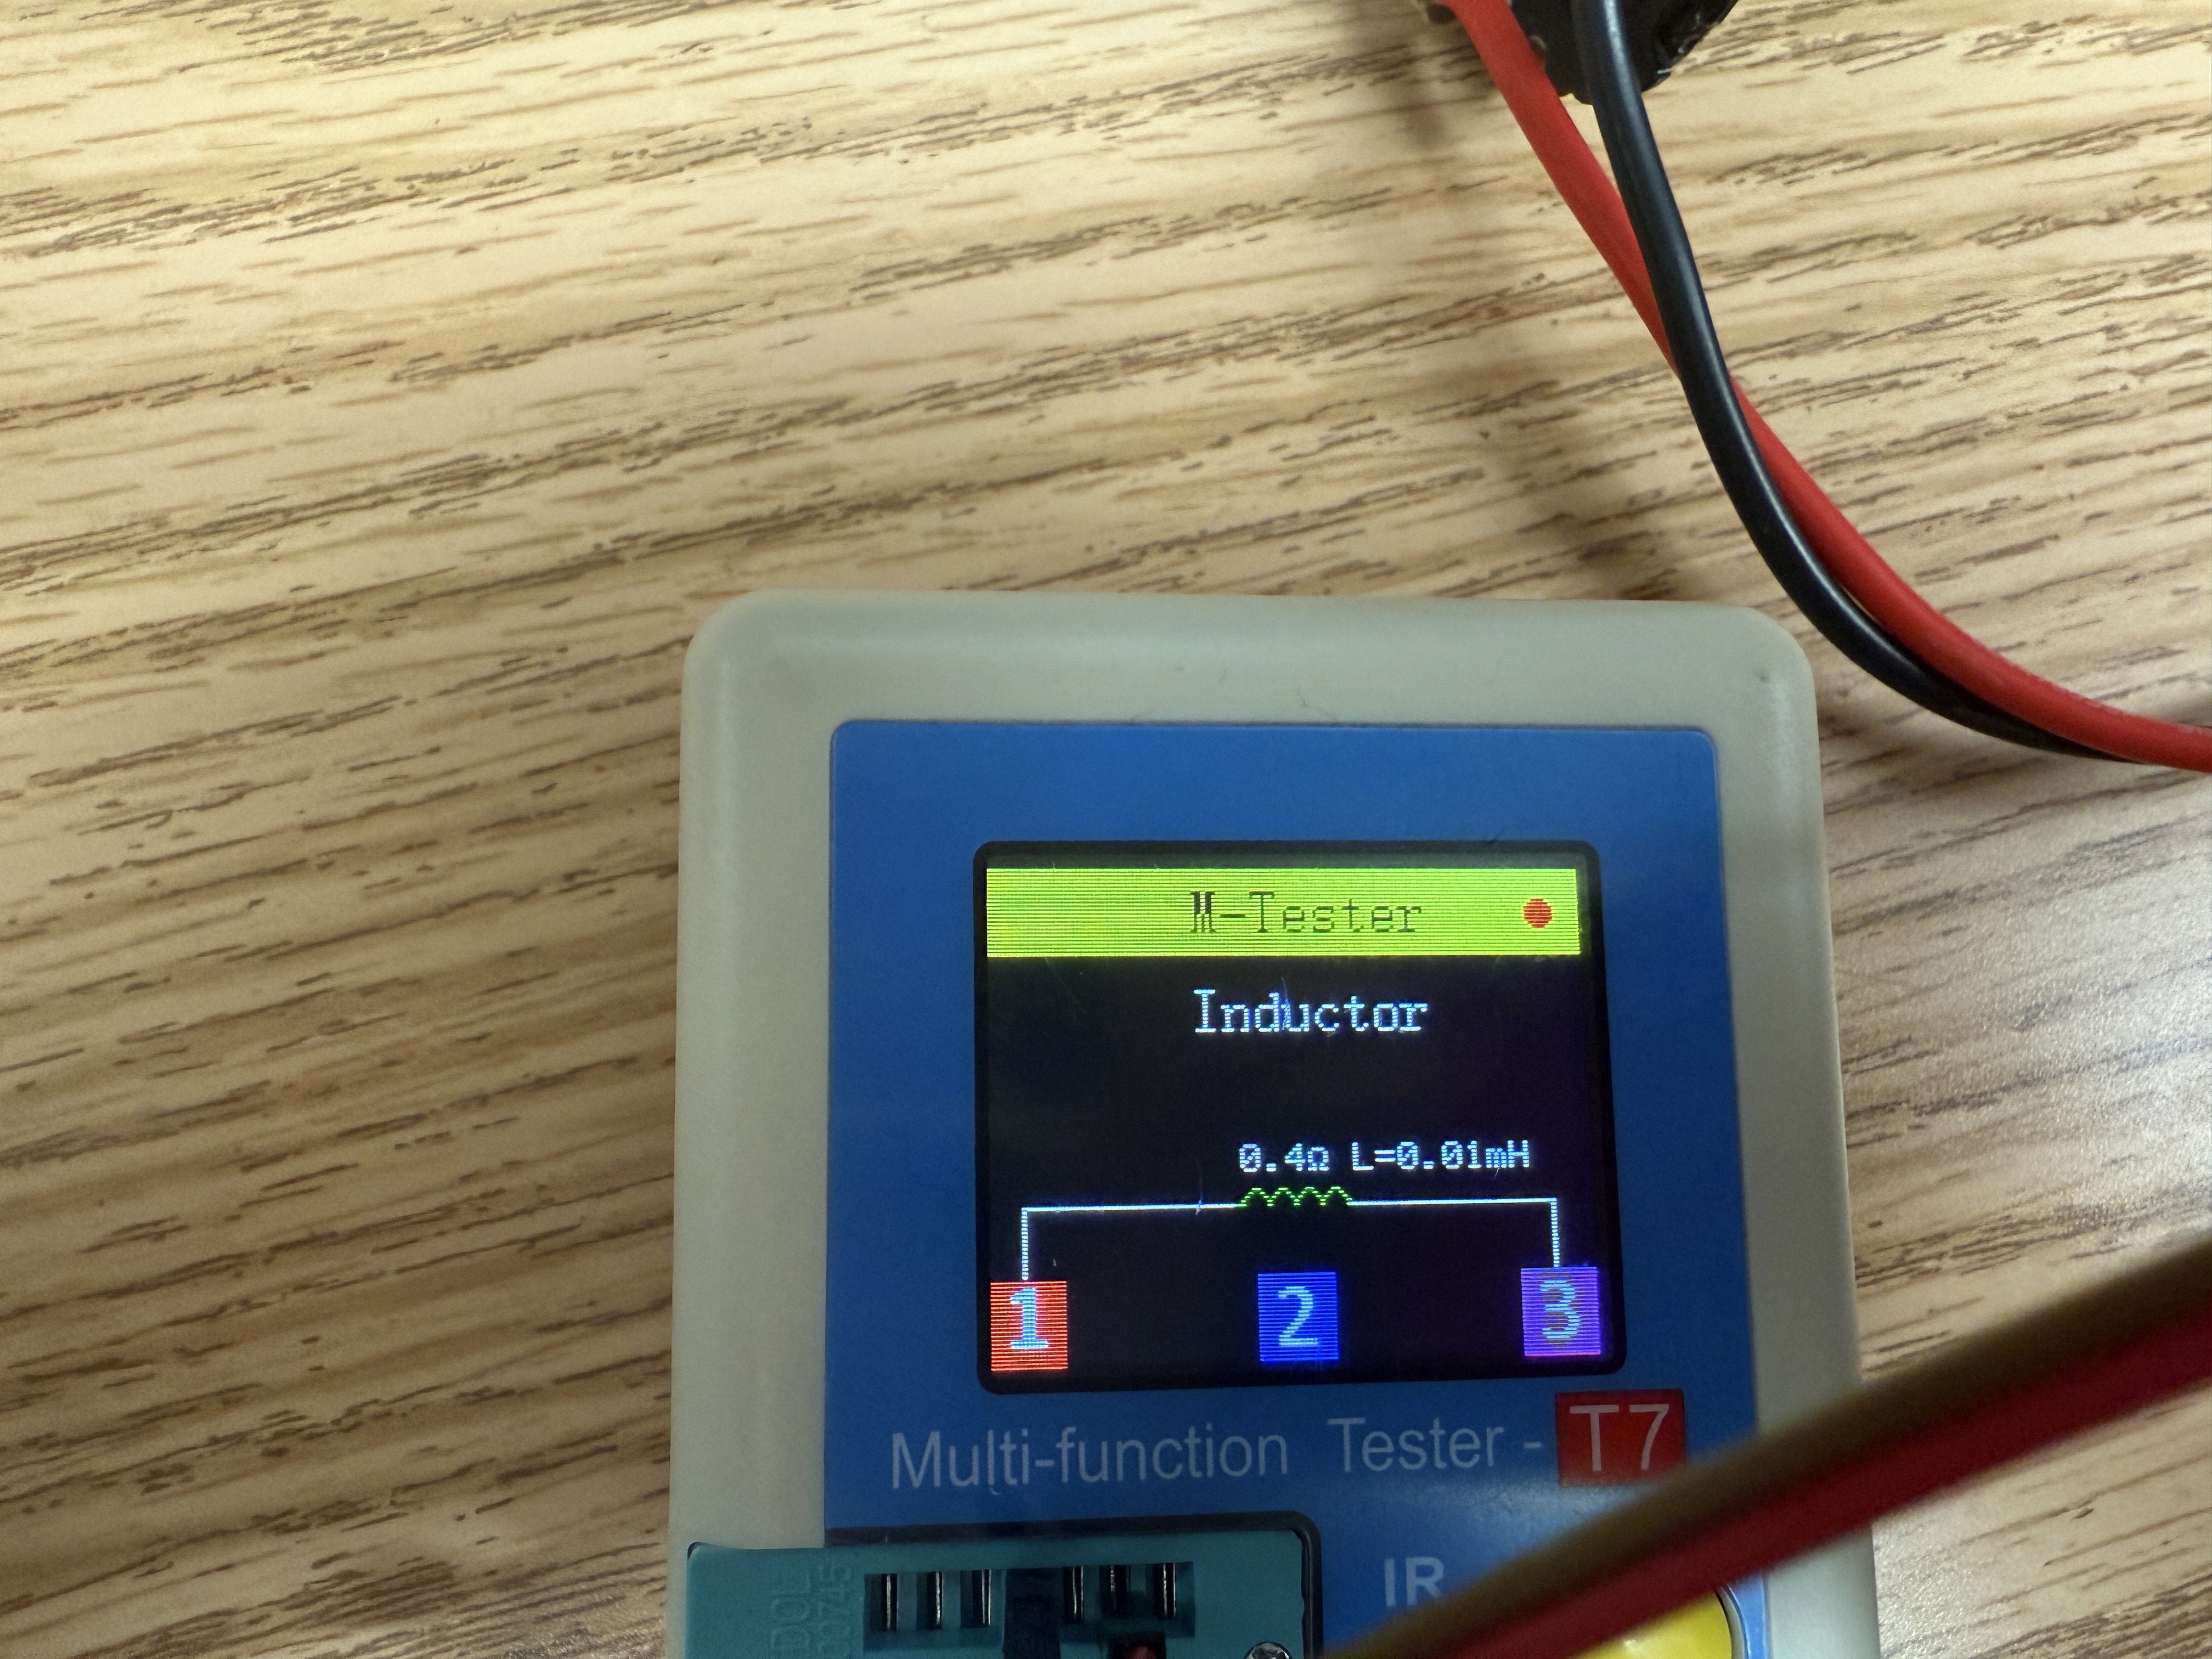
\includegraphics[width=0.8\textwidth]{images/Image.jpeg}
	\caption{Dyno testbench setup}
\end{figure}

	\item \textbf{Torque constant (Kt)}: Tested with values 100 Nm/A and 50 Nm/A to observe torque response.
	\item \textbf{Speed constant (Kv)}: Tested at 2000 rpm/V and 1000 rpm/V to assess speed-voltage behavior.
	\item \textbf{Mass and Inertia}: The mass of the Rotor, Flywheel, and Gears were measured to accurately capture the mechanical dynamics of the motor system. And the geometric inertia was captured directly from SolidWorks. These values are crucial for matching acceleration and deceleration behavior between simulation and experiment. This point applies to all the rotating bodies in the system.

\end{itemize}

\newpage\noindent
\textbf{Experimental Setup:} The motor was mounted on a custom-designed dyno testbench, which includes:
\begin{itemize}
	\item A flywheel (introduces inertia)
	\item A gear train (transmits motion)
	\item A secondary motor acting as a controllable load (dyno motor)
\end{itemize}

% \noindent
Tests were conducted with no load, constant load, and variable load conditions. Load types included constant torque values and sinusoidal torque waveforms. Data acquisition was performed at high-frequency sampling rates to ensure accurate capture of transient and steady-state motor behavior.

\section{\textbf{The Chrono Brushed Electric Motor \& Dyno Testbed Models}}
\begin{itemize}
    \needspace{10\baselineskip}
	\item \textbf{Brushed motor:} model captures electrical dynamics and electromechanical coupling using parameters extracted from measurements.
    \needspace{10\baselineskip}
	\item \textbf{Dyno Testbench:} modeled to simulate different load types including constant and time-varying torque.
\end{itemize}

\begin{figure}[H]
	\centering
	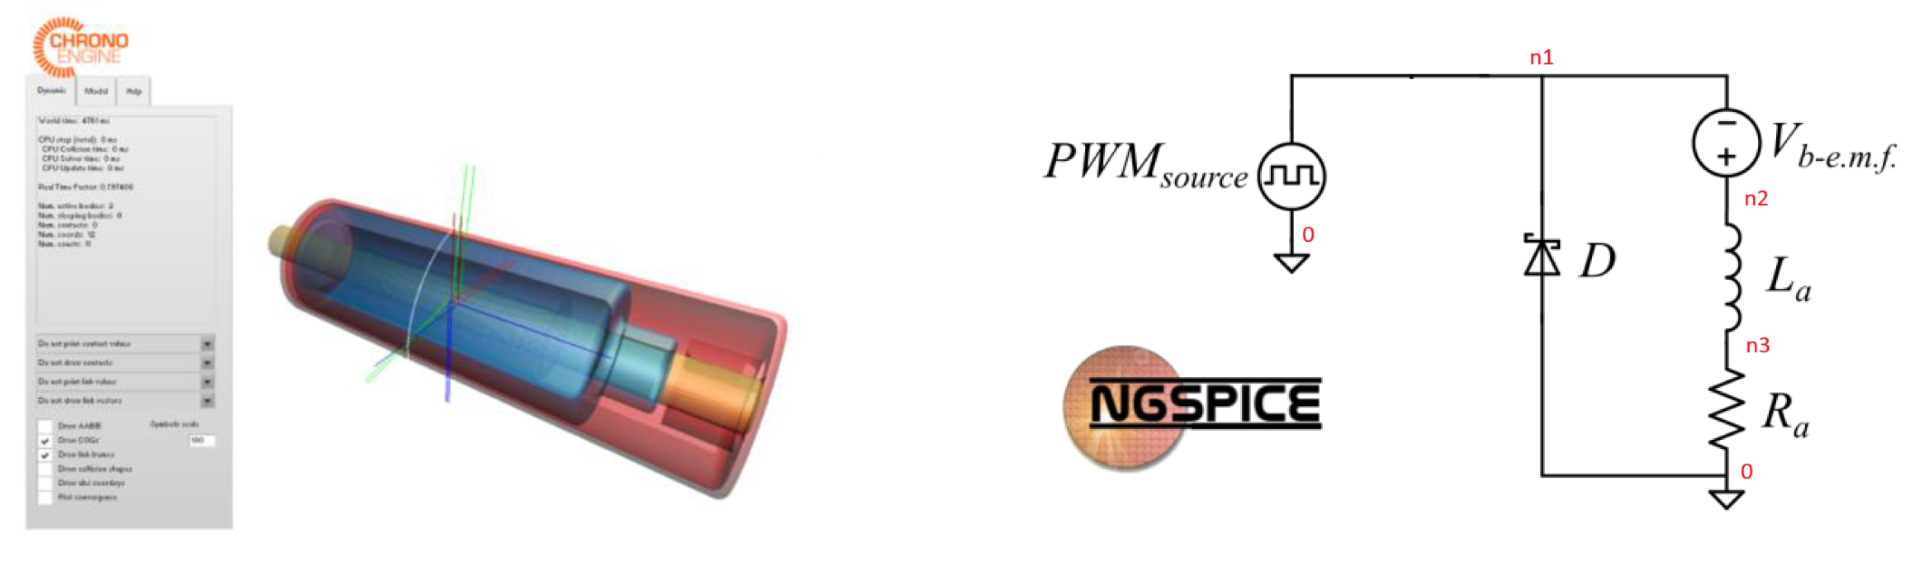
\includegraphics[width=1.0\textwidth]{images/thumbnail_image005.png}
	\caption{NGspice circuit model of the DC motor}
\end{figure}

SolidWorks models were created for both the motor assembly and the dyno testbench. These models provide detailed CAD-based data, including:

\begin{itemize}
    \needspace{10\baselineskip}
    \item \textbf{The Dyno model:}
    \begin{figure}[H]
        \centering
        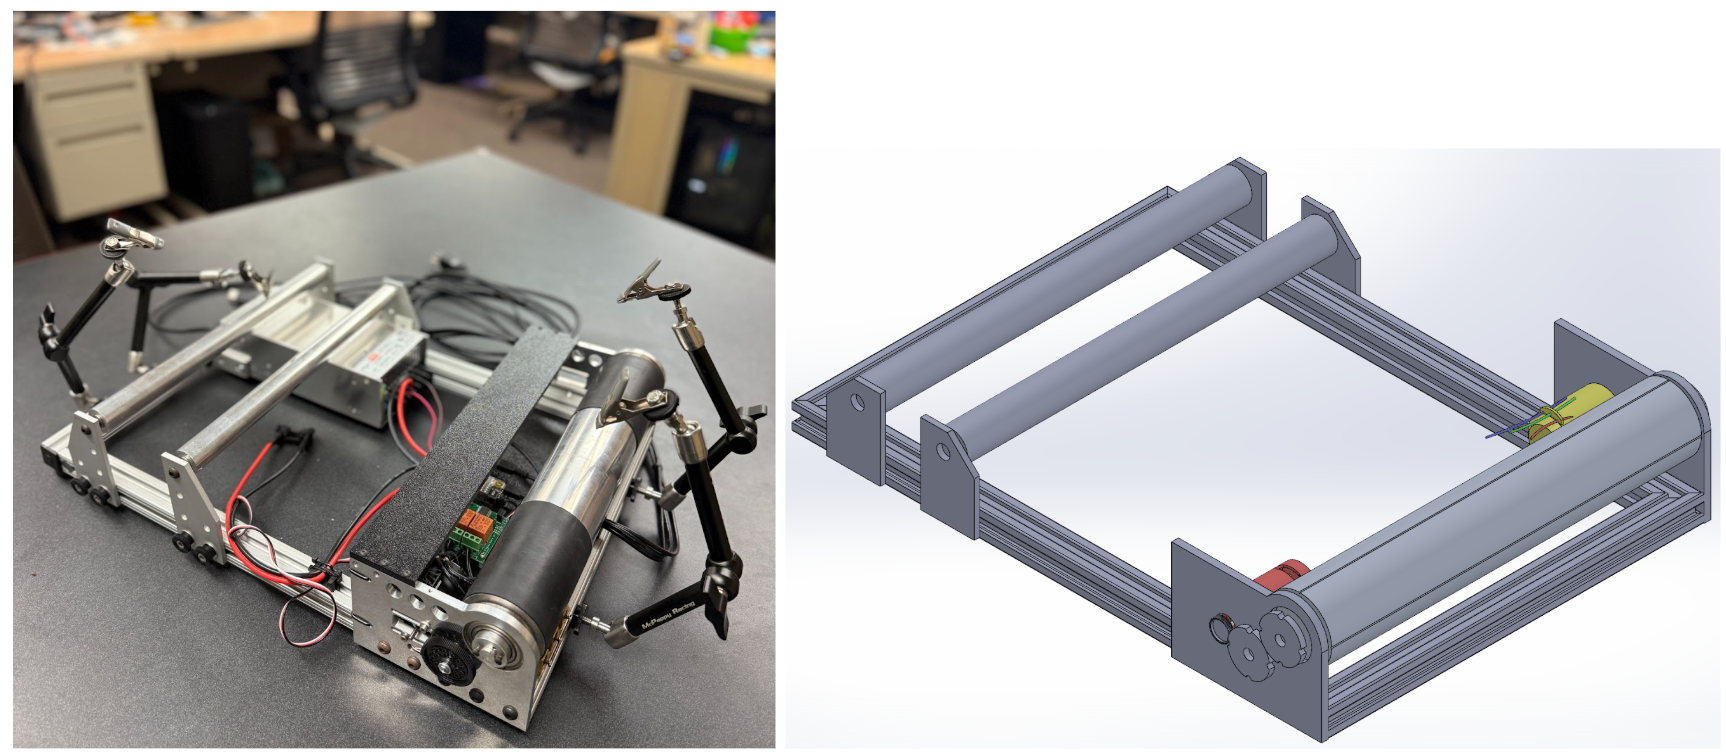
\includegraphics[width=1.0\textwidth]{images/Screenshot From 2025-03-26 04-25-26.png}
        \caption{NGspice circuit model of the DC motor}
    \end{figure}

    \needspace{5\baselineskip}
    \item \textbf{The Rotor and Rotor\_winding Model:}
    \begin{figure}[H]
        \centering
        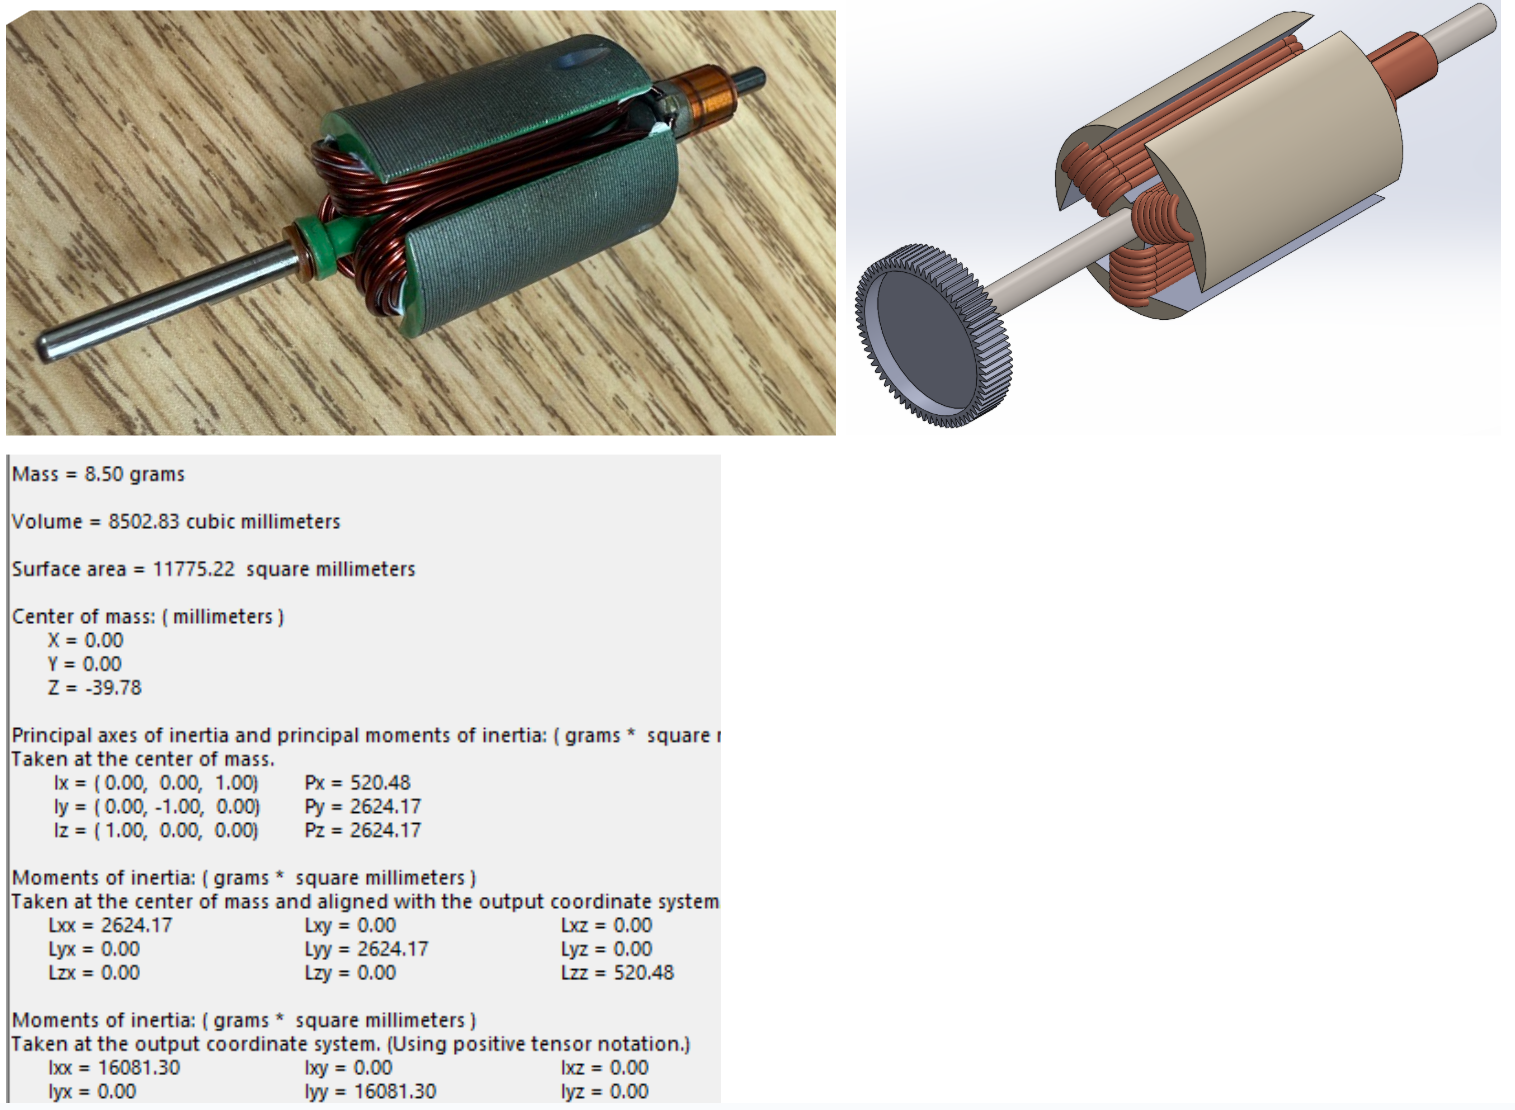
\includegraphics[width=0.8\textwidth]{images/Screenshot From 2025-03-26 04-26-15.png}
        \caption{NGspice circuit model of the DC motor}
    \end{figure}
\end{itemize}

\needspace{5\baselineskip}
\section{\textbf{\textbf{Plots to explain the Simulation parameters - }}}
\begin{itemize}
    \needspace{10\baselineskip}
	\item \textbf{Different rpm levels in response to the PWM input} 
        \begin{figure}[H]
        	\centering
        	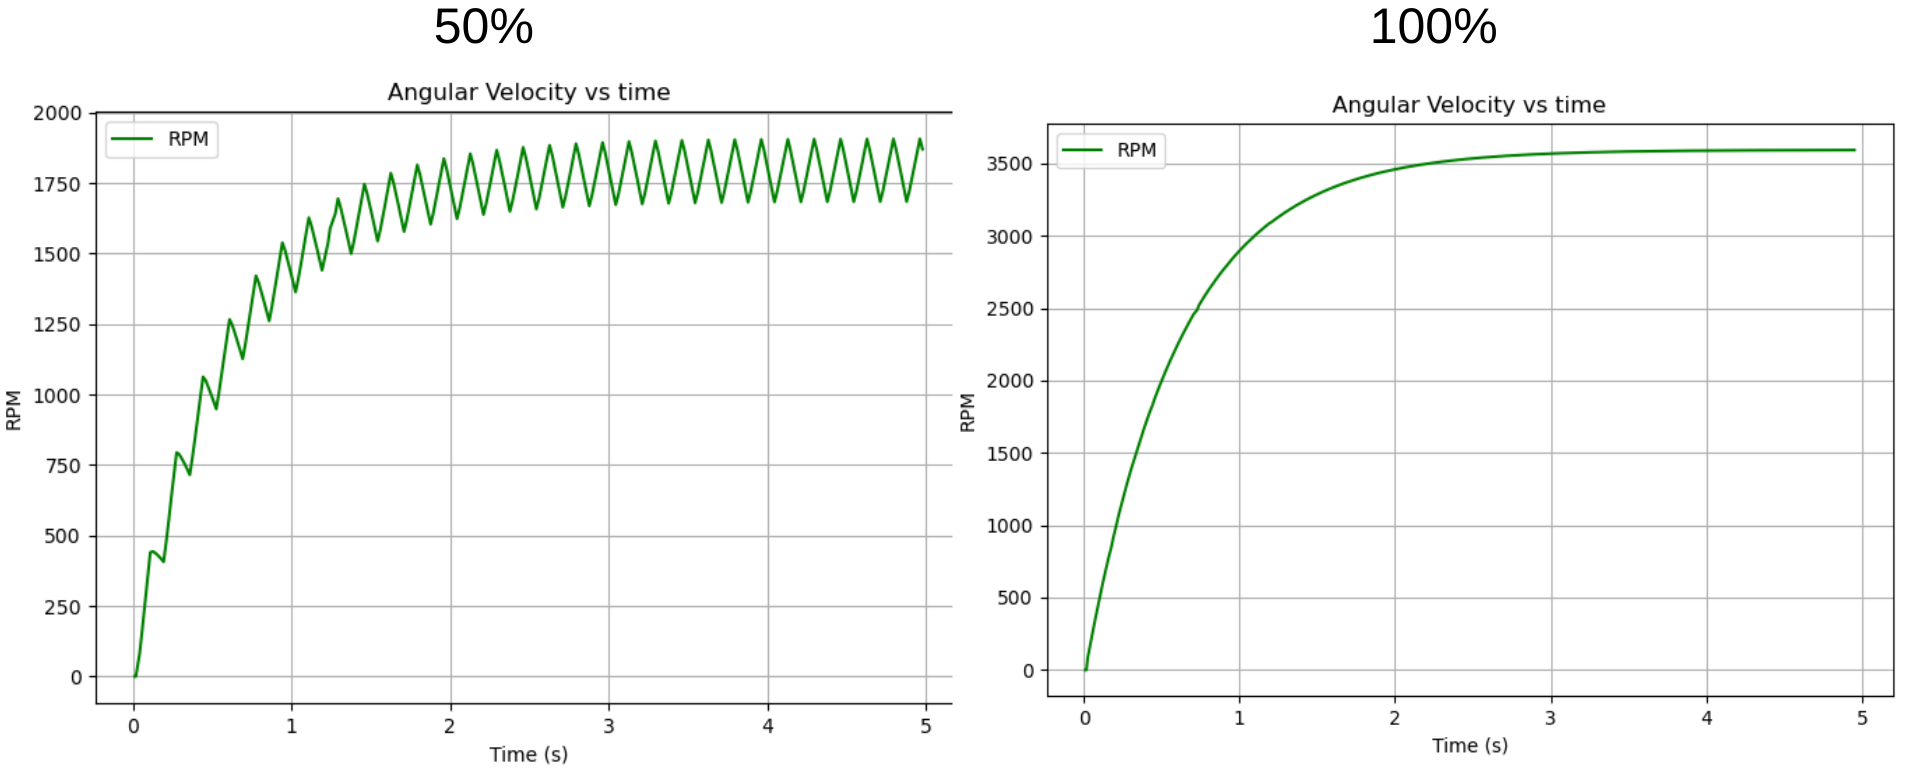
\includegraphics[width=1.0\textwidth]{images/Screenshot From 2025-03-26 07-08-18.png}
        \end{figure}

    \needspace{10\baselineskip}
	\item \textbf{Constant load torque application} 
        \begin{figure}[H]
        	\centering
        	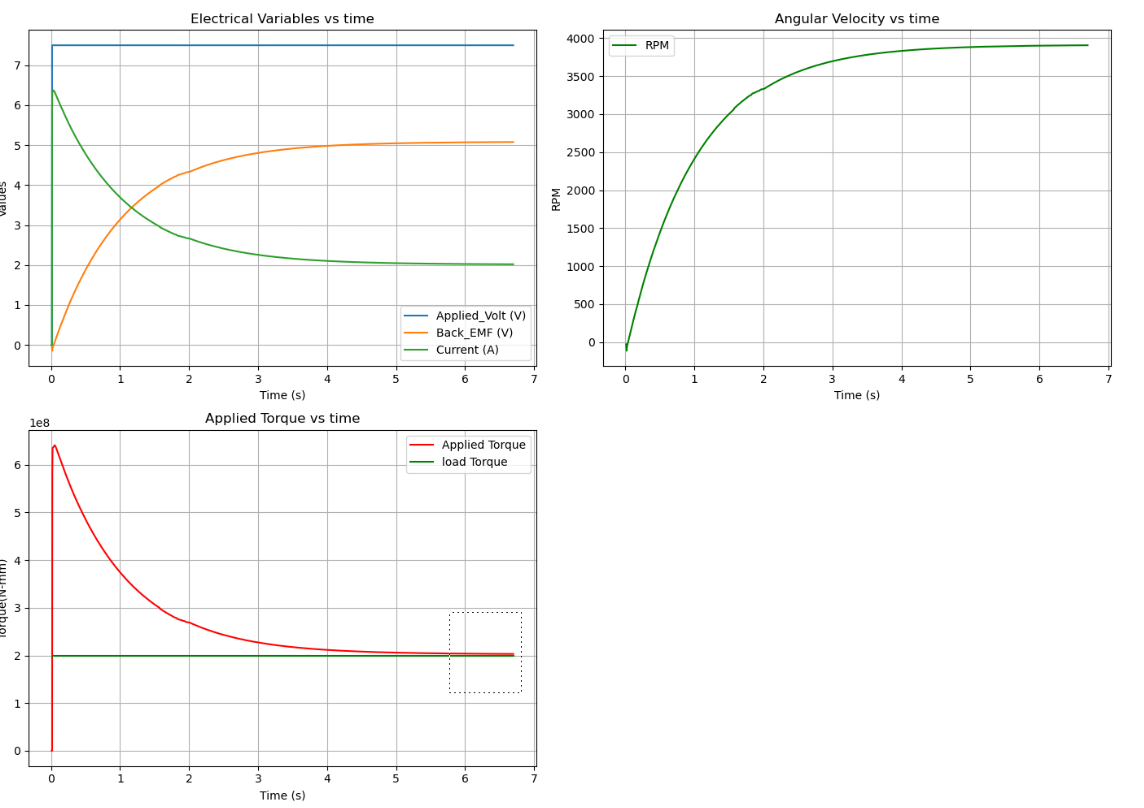
\includegraphics[width=1.0\textwidth]{images/Screenshot From 2025-03-26 03-23-59.png}
        \end{figure}

    \needspace{10\baselineskip}
	\item \textbf{Sinusoidal load torque application} 
        \begin{figure}[H]
        	\centering
        	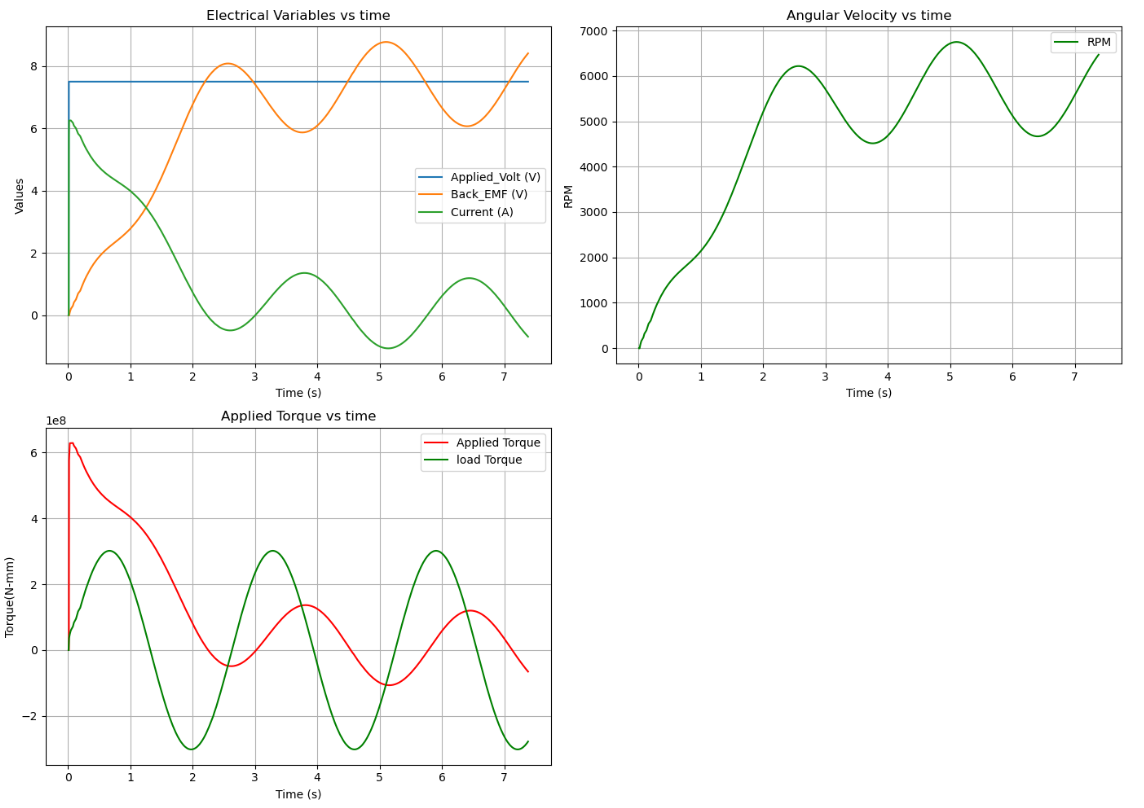
\includegraphics[width=1.0\textwidth]{images/Screenshot From 2025-03-26 03-35-23.png}
        \end{figure}

    \needspace{10\baselineskip}
	\item \textbf{The contribution of the Kt (Nm/A)} 
        \begin{figure}[H]
        	\centering
        	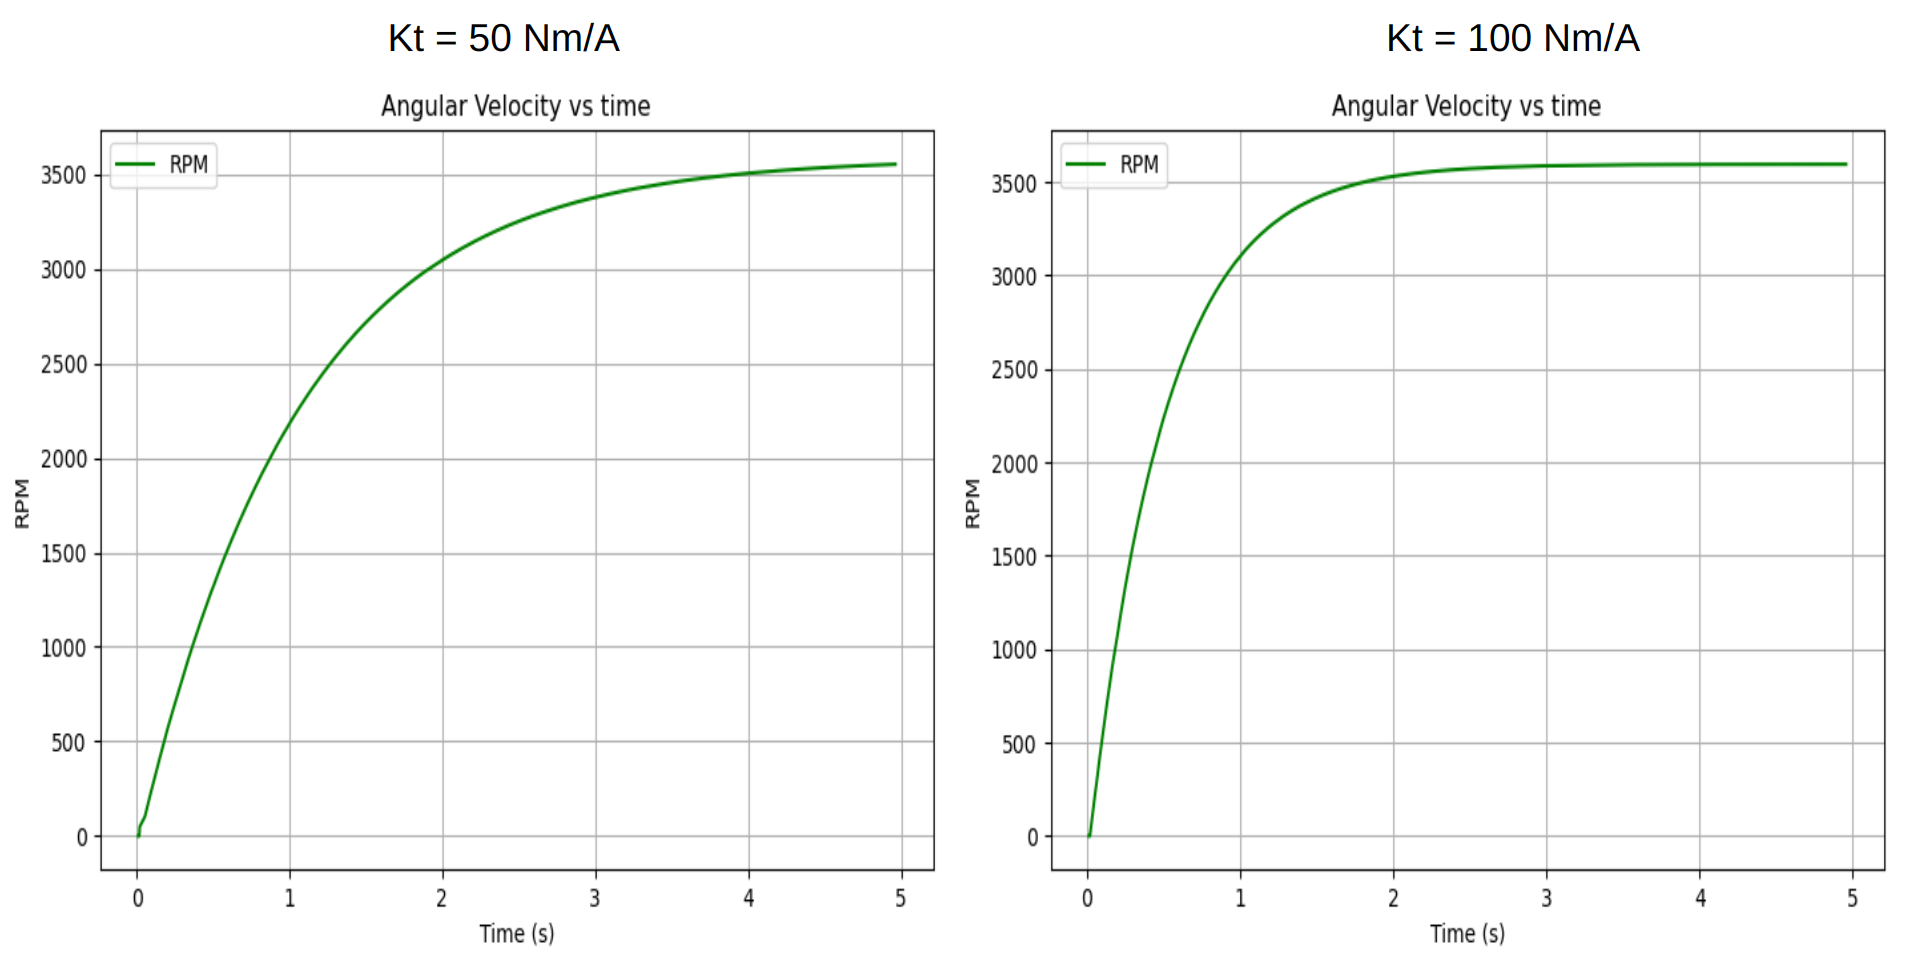
\includegraphics[width=1.0\textwidth]{images/Screenshot From 2025-03-26 07-11-42.png}
        \end{figure}

    \needspace{10\baselineskip}
	\item \textbf{The effect of the Kv (rpm/V)} 
        \begin{figure}[H]
        	\centering
        	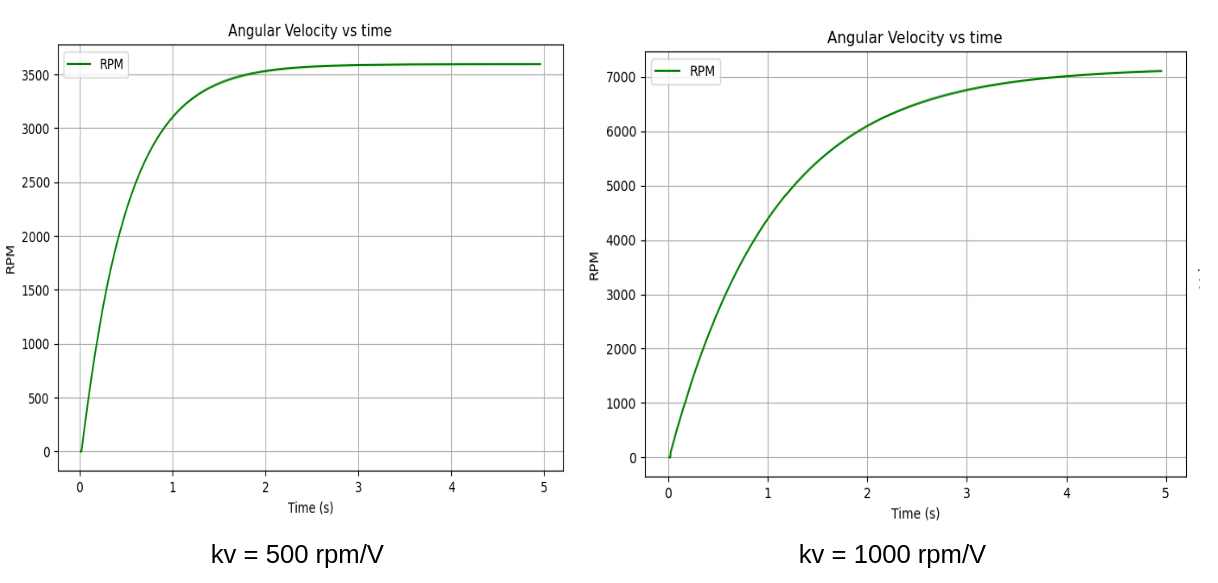
\includegraphics[width=1.0\textwidth]{images/Screenshot From 2025-03-26 03-44-11.png}
        \end{figure}

    \needspace{10\baselineskip}
    \item \textbf{Effect of SolverFrequency and SamplingTimestep on the PWM curve precision} 
        \begin{figure}[H]
            \centering
            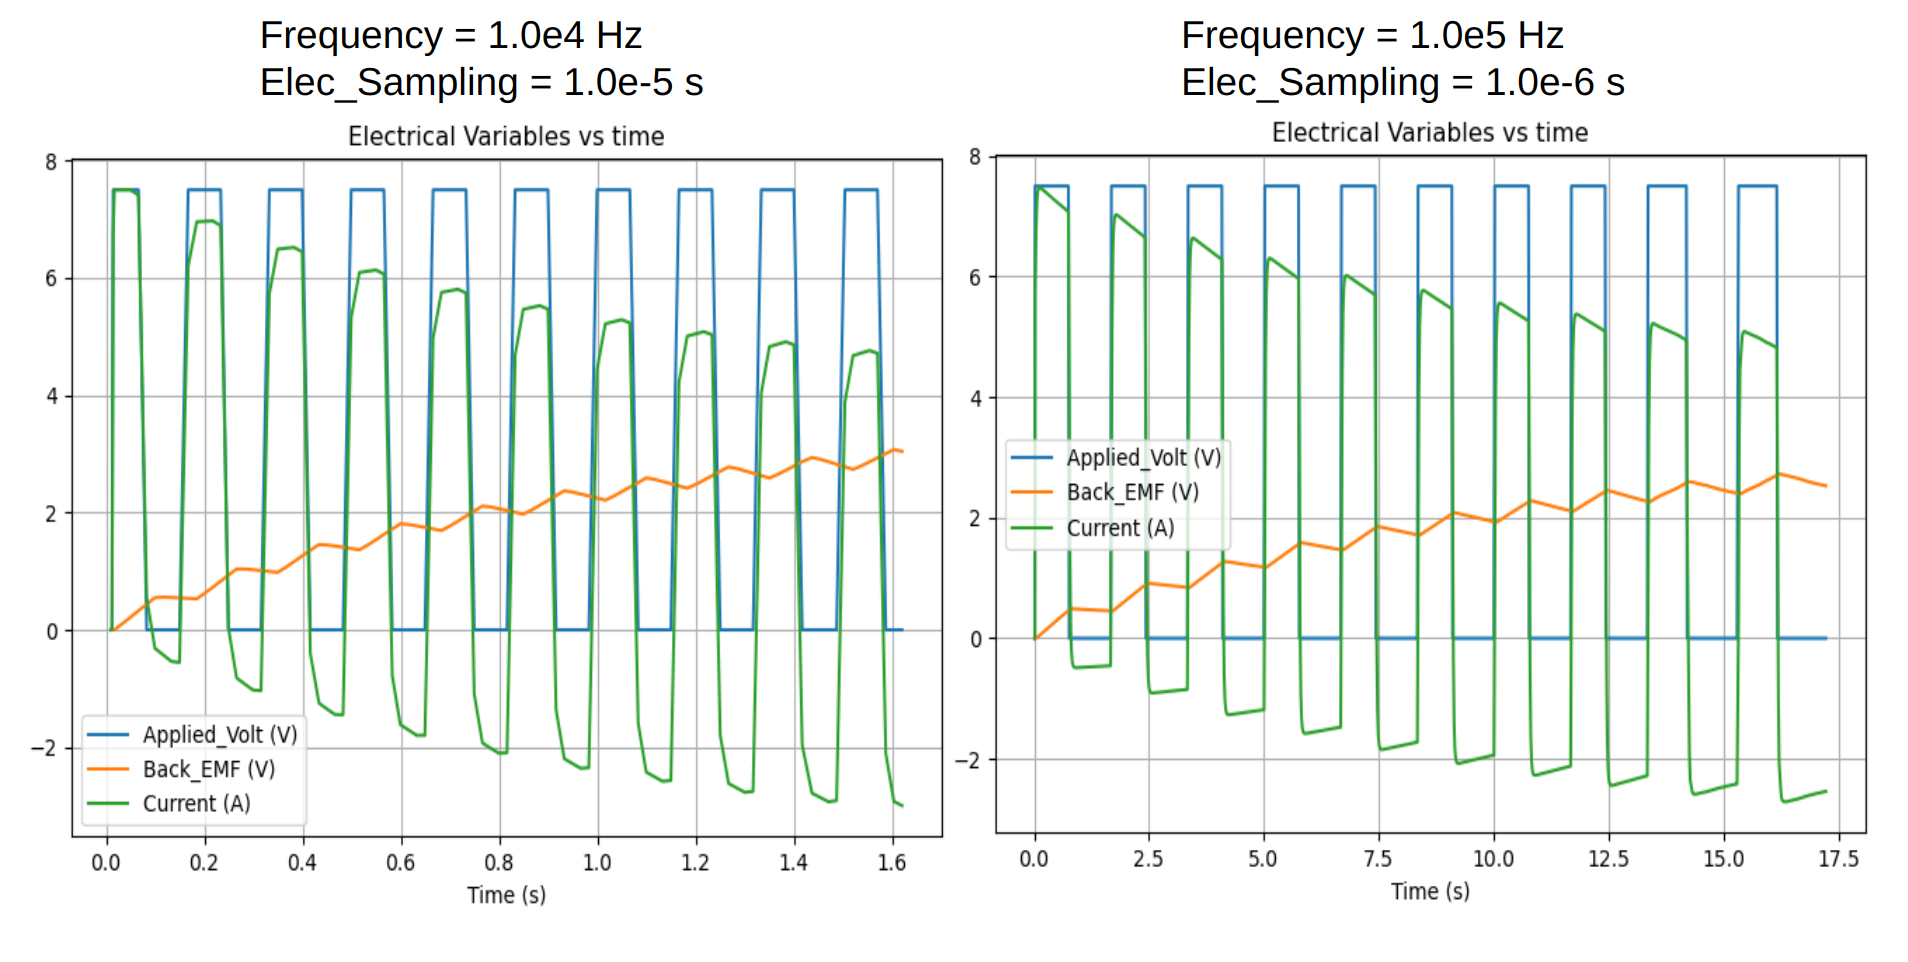
\includegraphics[width=1.0\textwidth]{images/Screenshot From 2025-03-26 07-13-48.png}
        \end{figure}
\end{itemize}



\newpage
\section{Validation study results}
\label{sec:numerical-results}
\begin{itemize}
    \needspace{10\baselineskip}
	\item \textbf{Simulation Methodology (Dyno Simulation):} \\
	Experimental data was exported into .csv file which was channeled to the chrono model. 
	Real time from the data was synchronized with the simulation timeStep to use the PWM Duty Cycle and the Load Torque as a input.

	All the crucial simulation Parameters used - 
	\begin{align}
	K_t &= 0.005\,\mathrm{Nm/A} \\
	K_v &= 1900\,\mathrm{rpm/V} \\
	\textit{Resistance} &= 0.040\,\Omega \\
	\textit{Inductance} &= 10 \times 10^{-5}\,\mathrm{H} \\
	\textit{PwmFrequency} &= 1\,\mathrm{kHz} \\
	\textit{MechanicalFrequency} &= 10^5\,\mathrm{Hz} \\
	\textit{ElectricalFrequency} &= 10^5\,\mathrm{Hz} \\
	\textit{ElectronicSamplingFrequency} &= 0.005\,\mathrm{Nm/A}
	\end{align}
	
	\begin{figure}[H]
		\centering
		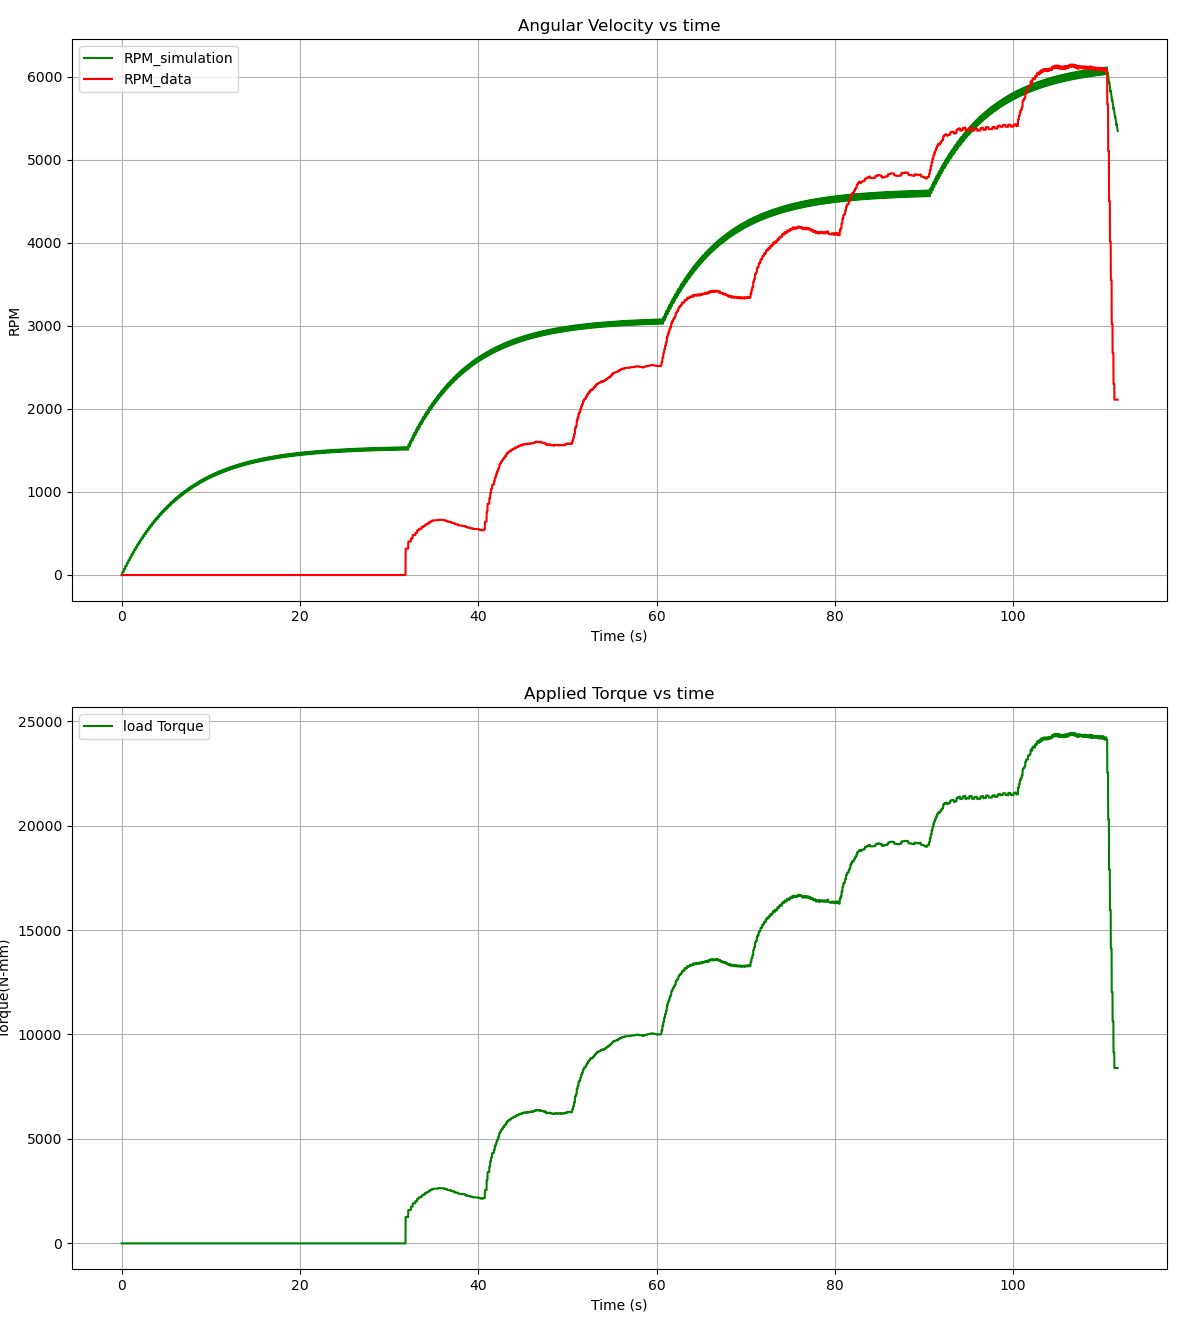
\includegraphics[width=0.75\textwidth]{images/Screenshot From 2025-03-26 07-59-40.png}
	\end{figure}
	\textbf{Observations-} \\
	As we can see the simulation can approximate the Dyno test data almost accurately with some errors. The error can be substantially decreased with further fine tuning of the frequencies, sampling time and the electical motor specifications.
	
    \needspace{10\baselineskip}
	\item \textbf{No load:} 
	
\end{itemize}
\begin{itemize}
	\needspace{10\baselineskip}
	\item Key comparisons include:
	\needspace{10\baselineskip}
	\item Motor speed (rpm) at 50% and 100% PWM
	\needspace{10\baselineskip}
	\item Impact of varying Kt and Kv
	\needspace{10\baselineskip}
	\item Torque response under different loading conditions
\end{itemize}

Plots were generated to compare experimental results with simulation outputs. These plots highlight the sim2real gap and show that simulation accuracy is sensitive to motor constants and load profiles.
An analytical estimate of error is currently under development, focusing on RMS differences and time-aligned errors over the testing duration.



\section{Conclusions and future Work}
\label{sec:futureWork}
To be added at the end.




% \section{Conclusion}
% \label{sec:conclusion}

\end{document}          